\chapter{Deep Reinforcement Learning for non-Markovian goals}

\label{ch:rl}

\section{Reinforcement Learning}

\label{sec:rl}

% Motivation
In this section, we will briefly review the most important aspects of classic
\emph{Reinforcement Learning} (RL). These concepts are relevant because they
are also found in Deep Reinforcement Learning (Deep RL), which is a central
component of the agent we will design. Excellent references for these topics
are \cite{bib:rl-book}, \cite{bib:probabilistic-rl}, and
\cite{bib:ml-book-murphy} for graphical models.

% Agent-env interface
In AI, we commonly isolate two entities, the agent and the environment, which
continuously interact. At each instant, the agent receives observations from
the environment and it executes actions in response. In RL specifically, the
agent observes the current state of the environment and a numerical reward.
The environment produces high rewards in response to desirable events. The
agent's goal is to maximize the rewards received. The basic setup is
illustrated in Figure~\ref{fig:rl}.

\begin{figure}
	\centering
	\begin{tikzpicture}
		\node [block] (agent) {Agent};
		\node [block, below=of agent] (env) {Environment};
		\draw [flow] ([yshift=2mm]env.west) -- ++(-1.2,0) |-
			([yshift=-2mm]agent.west) node [pos=0.3,right] {reward\\$r$};
		\draw [flow] ([yshift=-2mm]env.west) -- ++(-1.5,0) |-
			([yshift=2mm]agent.west) node [pos=0.3,left] {state\\$s$};
		\draw [flow] (agent.east) -| node [pos=0.7,right] {action\\a}
		($(env.east)+(1.2,0)$) -- (env.east);
	\end{tikzpicture}
	\caption{How agent and environment interact in RL.}
	\label{fig:rl}
\end{figure}


\subsection{Markov Decision Processes}

% MDP
Most RL algorithms assume that the environment dynamics can be modelled with a
\emph{Markov Decision Process} (MDP). They do so, because under the
independence assumptions taken by MDP, it's possible to efficiently find the
optimal agent's policy. A Markov Decision Process is a tuple $\langle \stateS,
A, T, R, \discount \rangle$, where: $\stateS$ is the set of states of the
environment; $A$ is the action space; $T: \stateS \times A \times \stateS \to
\R$ is the transition function, which, for ${T(s_{t}, a_{t}, s_{t+1})}$,
returns the probability $p(s_{t+1} \given s_{t}, a_{t})$ of the transition
${s_{t} \xrightarrow{a_{t}} s_{t+1}}$; $R: \stateS \times A \times \stateS \to
\R$ is the reward function; and $\discount \in [0, 1]$ is called ``discount
factor''\footnote{In this chapter, variables with an integer subscript or
index refer to the value at the discrete time indicated.}.

% Markov assumptions
In a RL problem, the functions $T$ and $R$ are unknown. The agent can only
learn them by taking each action and observing the outcomes. Even if they are
unknown, by assuming that they can be modelled with functions ${\stateS \times
A \times \stateS \to \R}$, we introduce some Markov assumptions. In
particular, we assume that the next state of the environment is conditionally
independent on the whole history, given the previous state and action:
$s_{t+1} \perp s_{0}, \dots, s_{t-1} \given s_{t}, a_{t}$. Similarly, the
reward only depends on the last transition of the environment.  Although it's
not required by the model, it is common that rewards are computed just from
desirable configurations of the environment~$s_{t}$, not from specific
transitions $(s_{t-1}, a_{t-1}, s_{t})$. All these assumptions are summarized
in the Directed Graphical Model (DGM) of Figure~\ref{fig:mdp}. In a DGM,
directed edges indicate direct conditional probabilities, while missing arcs
indicate conditionally independent variables.  In Figure~\ref{fig:mdp}, the
lack of any arrow between $s_{t-1}$ and $s_{t+1}$ means that future states,
hence the rewards, do not depend on the past history, given the current
state~$s_t$.  This is the essence of a Markov assumption.

\begin{figure}
	\centering
	\begin{tikzpicture}
		\matrix [
			column sep={1cm,between origins}, row sep={1cm,between origins},
		] {
			\&
			\node (am1) [node, label=above:$a_{t-1}$] {};
			\& \&
			\node (a) [node, label=above:$a_{t}$] {}; \& \\
			\node (stm1) [node, label=above:$s_{t-1}$] {};
			\& \&
			\node (st) [node, label=above:$s_{t}$] {}; \& \&
			\node (st1) [node, label=above:$s_{t+1}$] {}; \\
			\& \&
			\node (r) [node, label=below:$r_{t}$] {}; \& \&
			\node (r1) [node, label=below:$r_{t+1}$] {}; \\
		};
		\draw (st1) edge [<-] (st) edge [<-] (a);
		\draw [->, dotted] (st) -- (a);
		\draw [->] (st) -- (r);
		\draw [->] (st1) -- (r1);
		\draw (st) edge [<-] (stm1) edge [<-] (am1);
		\draw [->, dotted] (stm1) -- (am1);

		\draw [dashed, gray] (st1) -- +(0.8,0);
		\draw [dashed, gray] (stm1) -- +(-0.8,0);
	\end{tikzpicture}
	\caption{The directed graphical model of a MDP.}
	\label{fig:mdp}
\end{figure}

\begin{example}
	\label{ex:board-games}
	Tic-Tac-Toe, Chess and many other board games can be modelled with an MDP.
	Even games with dice, such as Backgammon. To do so, we define as state
	space~$\stateS$ the set of configurations of the board, and a reward
	function $R(s)$ that returns $1$, if the configuration $s$ is a win, $-1$
	for a loss, and 0 otherwise. Even though most games are deterministic, the
	presence of an opponent makes the transition function~$T$ of the MDP
	nondeterministic.  What these games have in common, is that the player gets
	to see the complete state of the game, which is the current configuration of
	the board. Future states of the game and rewards only depend on the current
	situation, not on the whole play. In Chess, for example, we can determine
	whether a configuration is a win or loss just by looking for a checkmate;
	there is no need to ask the players how the game has been carried out.

	Proving that Markovian $T$ and $R$ exist is easy for board games, because
	the rules of the game define them. As we will see in
	Section~\ref{sec:non-markov}, when $T$ is unknown, as always happens in the
	real-world, it's much more difficult to prove that we're in fact facing a
	MDP.
\end{example}


\subsection{Optimal policies}

The \emph{policy} is the criterion the agent uses to select the actions to
perform. If the environment dynamics can be modelled with a MDP, the
optimal action at time~$t$ only depends on~$s_{t}$. So, there must exist
an optimal policy as $\policy^*: \stateS \to A$. Due to common estimation
errors, it is always better to prefer nondeterministic policies, which return
a probability distribution over the actions. The action at time $t$ will be
sampled according to $a_t \sim \policy(s_t)$. This dependency is represented
by the dotted arrows of Figure~\ref{fig:mdp}.

We will now introduce few basic quantities of RL that serve to define what it
means for an action or a policy to be optimal. The \emph{discounted
return}~$G$ is the combination of all rewards collected:
\begin{equation}
	G \coloneqq r_{0} + \discount\, r_1 + \discount^2 r_2 + \dots =
	\sum_{t=0}^{T} \discount^{t} r_{t}
	\label{eq:return}
\end{equation}
The discount factor, $0 \le \discount \le 1$, decides the relative importance
of immediate and future rewards. Usually, this factor is strictly less than 1
because this stimulates the agent to achieve rewards as soon as possible.
It also produces a finite discounted reward, even for an infinite run, where
$T \to \infty$.  Since the environments we will experiment with are video
games, each play is an episode and the total number of steps in each episode
is finite.

It is now clear, that the optimal policy should always maximize the expected
discounted return. The \emph{value function} of a policy $\policy$ computes
this quantity from each state $s$:
\begin{equation}
	v_{\policy}(s) \coloneqq \E_{\policy}[G \given s_0 = s]
\end{equation}
which is the expected value of $G$, when the agent starts from state $s$
and it follows the policy~$\policy$. The notation $\E_{\policy}$ indicates
that the estimation assumes that the actions are sampled according
to~$\policy$. Finally, we can define the \emph{optimal policy} $\policy^*$ as
the one maximizing the value function at all states:
\begin{equation}
	\policy^*: \quad v_{\policy^*}(s) \ge v_{\policy}(s) \qquad \forall s \in
	\stateS, \quad \text{for all $\policy$}
\end{equation}
The typical Reinforcement Learning problem is to find the optimal policy for
an MDP with unknown $T$ and~$R$.

The \emph{action-value function} of a policy $\policy$ is a similar measure to
the value function:
\begin{equation}
	q_{\policy}(s, a) \coloneqq \E_{\policy}[G \given s_0 = s, a_0 = a]
\end{equation}
which also forces the first action to be~$a$. Since the agent can only observe
outcomes of single actions, this is usually a much more convenient form for
updating the estimate of the expected discounted return. Most important, the
optimal policy can be simply expressed as:
\begin{equation}
	\policy^*(s) = \argmax_{a \in A} q_{\policy^*}(s, a)
	\label{eq:opt-policy-q}
\end{equation}
So, instead of learning the optimal policy directly, we can learn the optimal
state-value function,~$q_{\policy^*}$ (also denoted with $q^*$). Fortunately,
we don't need $\policy^*$ to valuate $q^*$ because, assuming optimality, we
know it satisfies the Bellman optimality equation:
\begin{align}
	q^*(s, a) &= \E\, \bigl[ r_{t+1} + \discount \max_{a'} q^*(s_{t+1}, a')
	\given s_t = s, a_t = a \bigr] \\
	&= \sum_{s', r'} p(s', r' \given s, a) \,
	\bigl( r' + \discount \max_{a'} q^*(s', a') \bigr)
	\label{eq:q-bellman}
\end{align}
for any~$t$.

Many learning algorithms exist for estimating $q^*$. Briefly, on-policy
algorithms, estimate $q_\policy$ of the policy $\policy$ that is being used
and improved, $\policy \to \policy^*$; off-policy algorithms, instead, act
according to any exploration policy $\policy_e$ and directly estimate $q^*$.
Two famous algorithms in these classes are SARSA and Q-learning, respectively.
The one used in this thesis is derived from the latter.


\subsection{Exploration policies}

If $q^*$ were know, equation~\eqref{eq:opt-policy-q} would be enough to always
select the optimal action. Generalizing for any $q$, we call that the
\emph{greedy policy}, because it always selects the best action according to
$q$:
\begin{equation}
	\policy_q(s) \coloneqq \argmax_{a \in A} q(s, a)
	\label{eq:pol-greedy}
\end{equation}
Unfortunately, while learning, we only have a rough estimate of the optimal
function, ${\est{q} \approx q^*}$. Being greedy with respect to sub-optimal
values is dangerous, because the agent may deterministically select
actions that repeatedly lead to dead-ends.  To mitigate this issue, we can
choose some actions at random. The \emph{\eps-greedy policy} is defined as:
\begin{equation}
	\policy_{q,\epsilon}(s) \coloneqq
	\begin{cases}
		\text{random action $a \in A$}
		&\text{with probability $\epsilon$} \\
		\argmax_{a \in A} q(s, a)
		&\text{otherwise}
	\end{cases}
	\label{eq:pol-eps}
\end{equation}
More precisely, random actions are sampled from a uniform distribution over
the set of actions $A$. By making random moves, the agent might escape from
suboptimal environment configurations. If $\epsilon = 1$,
definition~\eqref{eq:pol-eps} reduces to the random policy:
\begin{equation}
	\policy_r(s) \coloneqq \text{random action $a \in A$}
	\label{eq:pol-random}
\end{equation}

When training begins, the agent has no clue about the optimal q-function. It
can just try out all actions by executing the random policy. In this phase,
the agent receives low rewards but observes a lot of different outcomes for
its actions. This is the purpose of exploration. After a while, the agent can
begin to trust in its predictions. So, it may gradually choose the most
promising actions in order to achieve higher rewards. This is the exploitation
phase.  The exploitation--exploration trade-off is a fundamental problem in
AI.  Unfortunately, there's no general solution in RL, because the agent has
no way to tell when the policy is ``good enough''. Usually, we need to try
some compromises between the two.

To address this issue, during training, the agent can act according to a
policy that is initially stochastic but gradually approaches the greedy
policy, over time. There are many ways to do this. One of the most simple
options is to select the \eps{}-greedy policy of equation~\eqref{eq:pol-eps}
with \eps{} that varies over time according to some schedule.
Figure~\ref{fig:policy-schedules} shows two common possibilities.
\begin{figure}
	\centering
	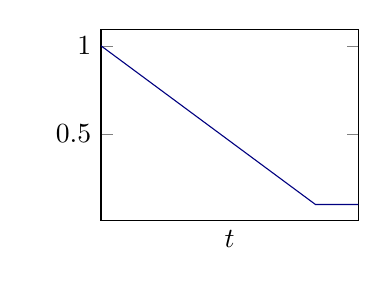
\begin{tikzpicture}
		\begin{axis}[
				xmin=0, xmax=120, width=0.4\textwidth, height=4cm,
				xlabel=$t$, ylabel=\eps{}, xtick=\empty]
			\addplot [blue!50!black] coordinates {
				(0, 1)
				(100, 0.1)
				(120, 0.1)
			};
		\end{axis}
	\end{tikzpicture}
	\qquad
	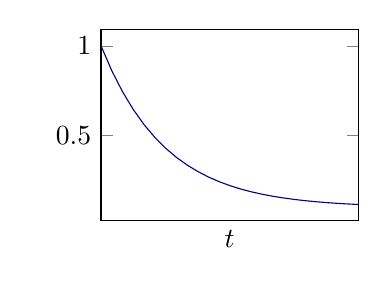
\begin{tikzpicture}
		\begin{axis}[
				xmin=0, xmax=120, width=0.4\textwidth, height=4cm,
				xlabel=$t$, ylabel=\eps{}, xtick=\empty]
			\addplot [blue!50!black, domain=0:120] {
				0.9*exp(-x/30)+0.1
			};
		\end{axis}
	\end{tikzpicture}
	\caption{Probability of a random action over time: \eps{} with linear decay
	(left), \eps{} with exponential decay (right).}
	\label{fig:policy-schedules}
\end{figure}
On the left-hand figure, the probability of a random action is linearly
decreased over time, while on the right, it follows an exponential decay. In
both cases \eps{} never becomes zero, because that would effectively terminate
the learning process. The rate of this decrease is a hyperparameter that
can be tuned.

The most important policies are those just described. They can be directly
used in a RL algorithm or combined to create more complex policies.  The
variants adopted in this thesis will be presented in the next chapters.  With
``exploration policy'' we refer to any policy that has a strong component of
nondeterminism and it's suitable to select the agent's actions during
training.


\section{Deep Reinforcement Learning}

\label{sec:deep-rl}

Classic RL algorithms, such as SARSA and Q-learning, are tabular methods.
In fact, they store and update the estimate for each pair $(s, a)$
independently. Unfortunately, this requires discrete and small states and
actions spaces. To overcome this very limiting assumption, we need
parametrized value functions and policies.  \emph{Deep Reinforcement Learning}
(Deep RL) is a recent field of RL in which Neural Networks (NN) are used as
powerful function approximators for policies or value functions.

The main advantage of NNs, and parametric models in general, is that they can
be trained in high-dimensional and continuous input spaces. In fact, a good
fit does not require a complete exploration of the input space, which may be
unfeasible or impossible. Instead, they are trained with some form of
Stochastic Gradient Descent (SGD) on the set of parameters from input-output
samples. Then, the model can be able to generalize to inputs that have been
never observed, in a meaningful way.

Unfortunately, due to approximation and parametrization, Deep RL algorithms
allow very little guarantees about convergence and optimality. Even if the
input space would be explored completely, updates for recent samples would
also affect the regions previously visited. In fact, any effective Deep RL
algorithm introduces some techniques in order to generate a stable training.


\subsection{Environment: Atari 2600 games}

The Atari 2600 is a video game platform that was developed in 1977. There are
hundreds of classic games available to play: Space Invaders, Ms. Pacman,
Breakout and many others. The screen is 160 pixels wide and 210 pixels high,
with 8-bits colour depth. The joystick has 9 positions (3 for each axis) and
one button, for a total of 18 possible actions. For this reason, we'll only
focus on RL methods for discrete action spaces.

The Arcade Learning Environment~\cite{bib:atari-games} is a simple interface
to the Atari 2600 emulator. It allows agents to play and be trained on these
games. At each step, the agent chooses one of the 18 actions available and
receives in return a frame of the game and a reward. The reward is the
increment in the player's score for the original game. This is really the same
interface that a human player would use. Figure~\ref{fig:atari-frames} shows
the frames from few games in this collection. 

\begin{figure}
	\centering
	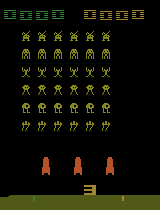
\includegraphics[width=0.25\textwidth]{./imgs/si0.png}
	\quad
	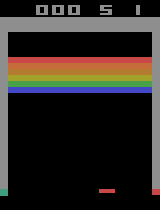
\includegraphics[width=0.25\textwidth]{./imgs/br0.png}
	\quad
	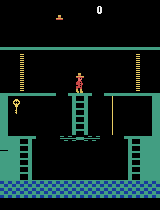
\includegraphics[width=0.25\textwidth]{./imgs/mz0.png}
	\caption{Initial frames of some Atari 2600 games (left to right): Space
		Invaders, Breakout, Montezuma's Revenge.}
	\label{fig:atari-frames}
\end{figure}

Although these games come from an early stage of video games development, they
represent the appropriate challenge for current (Deep) Reinforcement Learning
agents. In fact, many papers tested their RL algorithms on these
games~\cite{bib:atari-deeprl}%
\cite{bib:atari-deepq-nature}\cite{bib:double-q}\cite{bib:rainbow}.
In this thesis, we also tested with some of these environments. We will also
show how improve on the hardest game in this collection for a RL agent:
Montezuma's Revenge.


\subsection{Deep Q-Network}

The \emph{Deep Q-Network} (DQN)~\cite{bib:atari-deeprl} was the first
algorithm to successfully combine deep learning models and Reinforcement
Learning. Although many basic ideas presented here have been already
introduced by the Neural Fitted Q~iteration algorithm~\cite{bib:nfq}, DQN
addressed some causes of training instability. They also demonstrated that
exactly the same agent can be trained in many Atari games and achieve
human-level performances in many of those~\cite{bib:atari-deepq-nature}. These
promising results sparked a lively interest in Deep RL, recently.

In DQN, the state-action value is approximated by a deep neural network ${Q(s,
a; \params)}$, on the parmeters $\params$, that we call Q-Network. The purpose
of learning, is to train this network to approximate the optimal q-function: 
$\est{\params}: Q(s, a; \est{\params}) \approx q^*(s, a)$. Then, the estimated
optimal policy will be:
\begin{equation}
	\est{\policy}(s) = \argmax_{a \in A} Q(s, a; \est{\params})
\end{equation}

A trained network, for each input $(s, a)$, should return the expected value
of some target~$y_{s,a}$. To do so, we select the parameters that minimize the
squared difference between the estimates and the targets:
\begin{equation}
	\text{loss}(\params) \coloneqq \bigl(Q(s, a; \params) - y_{s,a} \bigr)^2
	\label{eq:qnet-generic-loss}
\end{equation}
Since this is a Q-Network, the targets are the optimal state-action
values~$q^*(s, a)$ that the net should estimate.  The
loss~\eqref{eq:qnet-generic-loss} contains some random variables. So, we
minimize it through any stochastic optimization algorithm. In Stochastic
Gradient Descent (SGD), at each step $t$, we observe an input ${(s_t, a_t)}$
and the associated target $y_t$. Then, we take a small step toward the
negative gradient of the loss:
\begin{equation}
	\params_{t+1} = \params_t - \alpha\, \nabla_{\params}\,
	\Bigl( \bigl(Q(s_t, a_t; \params) - y_t \bigr)^2 \Bigr) \Big|_{\params =
	\params_t}
	\label{eq:sgd-update}
\end{equation}
in which $0 < \alpha < 1$ is a small learning rate. This equation is not
the only update rule possible. There are more advanced optimization
algorithms, such as: Momentum, RMSprop and Adam. In this thesis, we've
mostly experimented with Adam.

What has just been described is the usual way of fitting a neural network
to a dataset of samples. In RL, however, the targets $q^*(s_t, a_t)$ are
unknown, because they depend recursively from the same optimal q-function
that we're trying to learn (see equation~\eqref{eq:q-bellman}). In classic RL,
this is not a problem: the 1-step approximation of the q-values (derived from
equation~\eqref{eq:q-bellman}),
\begin{equation}
	y_t \coloneqq r_{t+1} + \discount \max_{a \in A} \est{q}(s_{t+1}, a)
	\label{eq:1step-targets}
\end{equation}
or the n-step approximation, are a valid targets for the function~$\est{q}$.
By updating toward these values on the whole input space, convergence is
guaranteed. In other words, targets can be estimates themselves.

With neural networks, instead, any update to the parameters also affects the
target, because the weights have a global influence on the function. It's not
possible apply a correction for just one tiny region of the input space (nor
it's desirable, after all).  It has been shown~\cite{bib:nfq}, that due to
this effect, propagating errors slow down convergence or even render the
training unstable.  To address this issue one must ensure that the targets do
not move much.

The DQN~\cite{bib:atari-deeprl} algorithm addresses this issue in two ways.
First, the targets in equation~\eqref{eq:1step-targets} are not generated by
the network that is being trained, $Q(s, a; \params)$, but they are computed
from a second net, $Q(s, a; \params')$. Every $C$ iterations, the target net
is updated to match the trained net, with the assignment: $\params' \gets
\params$. This keeps the targets constant for $C$ steps and helps to stabilize
the training.

Second, the network is not trained from the last sample, but from transitions
of the recent experience. At each step, the agent acts according to some
exploration policy, $a_t \sim \policy_e$. Each transition, of the form
$\langle s_t, a_t, r_{t+1}, s_{t+1} \rangle$, is recorded in a buffer of size
$n_r$, called ``experience replay''. Then, at each training step, we sample a
number of $n_b$ transitions, thus creating a batch, and we perform an update
$\params_{i+1} = \params_i - \alpha\, g_i$ on the cumulative gradient $g_i$ of
the whole batch.

DQN also includes a number of heuristics that greatly help the training
but are specific to the Atari~2600 environments:
\begin{itemize}
	\item Rewards can be really high, so they are limited in the range $[-1,
		+1]$; this is called \emph{reward clipping}. It helps to keep the same
		learning rate for diverse games.
	\item The agent has a single life available. When a life is lost, the
		episode ends. This prevents the agent to rely on restarts.
	\item The frames are slightly down-scaled to further reduce the resolution,
		they are transformed to gray-scale and mapped to the range $[-1, +1]$.
		These are common preprocessing steps for NNs.
	\item Every observation is composed by the last 4 frames stacked together.
		This allows the agent to observe how the objects in the scene move.
		See Section~\ref{sec:non-markov} and Example~\vref{ex:motion}.
\end{itemize}

The algorithm used in this thesis is called \emph{Double
DQN}~\cite{bib:double-q}. It is a slight variant of DQN, so all details
mentioned so far also apply. The motivation of this algorithm is a known issue
of Q-learning: it is likely to make overoptimistic value estimates.
To show this, let's rewrite the targets of~\eqref{eq:1step-targets} as:
\begin{equation}
	y_t \coloneqq r_{t+1} + \discount \, Q(s_{t+1}, \argmax_{a \in A} Q(s_{t+1},
	a; \params_t); \params_t)
\end{equation}
where the estimates $\est{q}$ are computed with the Q-Network. This form makes
more evident that the same model is used both to select the next greedy action
and to estimate the q-value of state~$s_t$. As result, any action with an
overestimated q-value will be selected and its value propagated. To remove
this bias, Double DQN decouple the two operations by using different sets of
parameters, $\params\group{1}$ and $\params\group{2}$. The targets $y_t$ are
computed as:
\begin{equation}
	y_t \coloneqq r_{t+1} + \discount \, Q(s_{t+1}, \argmax_{a \in A} Q(s_{t+1},
	a; \params_t\group{1}); \params_t\group{2})
	\label{eq:double-q-targets}
\end{equation}
Then, just the parameters $\params\group{1}$ are updated toward this targets;
this is called the online network. With random chance, the roles of the two
parameters are continuously swapped at each step.

To compute the target, we need to compute the q-values for all actions in
state $s_{t+1}$. To speed up this computation, the network is defined as a
function that takes in input a state and computes a vector of state-action
values, one for each action. So, just one forward pass is required to select
the next action. Common Q-Networks for images are composed of a number of
convolutional layers and some fully-connected layers. The specific structure
may change, and the network used will be defined in the implementation section.


\section{Non-Markovian goals}

\label{sec:non-markov}

The goal of a RL agent is to maximize the rewards received.  A goal, or a
task, is said \emph{non-Markovian} if the rewards do not satisfy the Markov
assumption on rewards, i.e:
\begin{equation}
	r_{t+1} \not\perp s_t, a_t, r_t \quad 0 \le i < t \qquad \text{for some $t$}
	\label{eq:markov-rewards}
\end{equation}
% TODO: the above equation should have o_t not s_t, notation?
Of course, this can happen only if the environment cannot be modelled with an
MDP. Excellent algorithms exists for MDPs; instead, non-Markovian goals are
much more difficult to learn.  There are two main causes for non-Markovian
rewards: partial observations and temporally-extended tasks. We'll thoroughly
analyze both scenarios.


\subsection{Partial observations}

Up to this point, we didn't need to distinguish between observations and
states. In fact, we assumed that the agent can directly observe the
environment states and act accordingly (we defined the policy as a function of
the state). Unfortunately, this is often not the case: we only get to see
something that depends on the current state, but it's not. These systems can
be modelled with a \emph{Partially Observable Markov Decision Process}
(POMDP).  POMDPs are a generalization of MDPs for partial observations. From
now on, we will denote with $\stateS$ the environment state space and with
$\obsS$ the observation space. Formally, a discrete-time POMDP is a 7-tuple
${\langle \stateS, A, T, R, \obsS, O, \discount \rangle}$, where $\stateS, A,
T, R$ are defined as usual, $\obsS$ is the observation space, and $O$ is the
observation function ${O: S \to \obsS}$.

The graphical model of a POMDP is shown in Figure~\ref{fig:pomdp}.
\begin{figure}

	\centering
	\begin{tikzpicture}
		\matrix [
			column sep={1.5cm,between origins}, row sep={1cm,between origins},
			hidden node/.style={node, fill=gray},
		] {
			\node (om1) [node, label=above:$o_{t-1}$] {}; \&
			\node (am1) [node, label=above:$a_{t-1}$] {}; \&
			\node (o) [node, label=above:$o_{t}$] {}; \&
			\node (a) [node, label=above:$a_{t}$] {}; \\
			\node (stm1) [hidden node, label=below left:$s_{t-1}$] {};
			\& \&
			\node (st) [hidden node, label=below left:$s_{t}$] {}; \& \&
			\node (st1) [hidden node, label=below left:$s_{t+1}$] {}; \\
			\& \&
			\node (r) [node, label=below:$r_{t}$] {}; \& \&
			\node (r1) [node, label=below:$r_{t+1}$] {}; \\
		};
		\draw [->] (stm1) -- (om1);
		\draw [->] (st) -- (o);
		%
		\draw [->] (st) -- (r);
		\draw [->] (st1) -- (r1);
		%
		\draw [->, dotted] (om1) -- node [midway] {?} (am1);
		\draw [->, dotted] (o) -- node [midway] {?} (a);
		%
		\draw (st) edge [<-] (stm1) edge [<-] (am1);
		\draw (st1) edge [<-] (st) edge [<-] (a);

		\draw [dashed, gray] (st1) -- +(0.8,0);
		\draw [dashed, gray] (stm1) -- +(-0.8,0);
	\end{tikzpicture}
	\caption{The Directed Graphical Model of a POMDP. Gray nodes are
	unobservable. For simplicity, the rewards in this graph depend just on the
	current state $s_t$, not on transitions ${(s_t, a_t, s_{t+1})}$.}
	\label{fig:pomdp}
\end{figure}
The sequence of states ${\langle s_0, s_1, \dots \rangle}$, which is the
environment dynamics, still satisfies the Markov assumption (it forms a Markov
chain). In a POMDP, this dynamics exists but is unobservable. What we can
see, instead, is a sequence of observations ${ \langle o_0, o_1, \dots
\rangle}$. Each of them is generated from the corresponding state, through the
(possibly nondeterministic) observation function. Actions and policies can
only act in response to observations, not states.

The dotted arrows in Figure~\ref{fig:pomdp} have a question mark on them,
because that dependency is our choice. As designers, we're free to select
the informations that the agent should take into account when selecting an
action. Is the last observation enough to decide? Or, more precisely, among
all possible policies, do non-Markovian goals always admit an optimal policy
of the form $\policy^*: \obsS \to A$? Unfortunately, the answer is no. As we
will see, other informations are needed.

If the transition and observation functions are known, a common solution is to
estimate the states and decide the action from this belief. With deterministic
functions, the agent can iteratively restrict the set of possible states by
eliminating those inconsistent with the observations received. More commonly,
these functions are nondeterministic. In this case, a probabilistic methods
can be effective estimation algorithms. The iterative probabilistic filter
applied to the sequence of observations would produce the belief distribution
on the current state.
We can represent the general procedure, at any instant~$t$, with the
following computation:
\begin{center}
	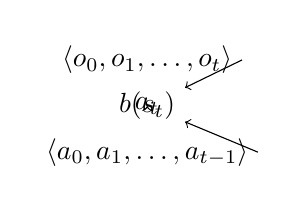
\begin{tikzpicture}
		\matrix [column sep=2em] {
			\node (o) {$\langle o_0, o_1, \dots, o_t \rangle$}; \\
			\&
			\node (s) {$b(s_t)$}; \& \node (an) {$a_t$}; \\
			\node (a) {$\langle a_0, a_1, \dots, a_{t-1} \rangle$}; \\
		};
		\draw [->] (o.east) -- (s);
		\draw [->] (a.east) -- (s);
		\draw [->] (s) -- (an);
	\end{tikzpicture}
\end{center}
where $b(s)$ denotes the belief of $s$, being either a set of states or a
probability distribution. Since each state estimate depends on the whole
sequence of observations, also the next action is implicitly based on the
whole history.

Standard RL algorithms cannot be applied to POMDPs, because the state space is
not observable. Also, since we commonly assume the transition and observation
functions to be unknown, no estimation could be carried out anyway.  There is
a clear difference between MDPs and POMDPs. Still, RL algorithms are
frequently applied to POMDPs. Not surprisingly, they perform very poorly on
these environments. See, for example, the games with worst performances
in~\cite{bib:atari-deepq-nature}. This is a subtle mistake, because
determining whether we're observing the state space is the same as answering
the following question: does the observation space capture the whole dynamics
of the system? Or, more precisely, does an equivalent MDP $\langle \obsS, A,
T_\obsS, R_\obsS, \discount' \rangle$, that produces the same rewards, exist?
If both $T_\obsS: \obsS \times A \times \obsS \to \R$ and $R_\obsS: \obsS
\times A \times \obsS \to \R$ exist and produce the same rewards, the
environment can be successfully modelled and solved with an MDP.
Figure~\ref{fig:pomdp-as-mpd} represents this situation.

\begin{figure}
	\centering
	\begin{tikzpicture}[
			hidden node/.style={node, fill=gray},
			hidden arc/.style={->, densely dotted},
			box/.style={rounded corners=5pt, inner sep=1.8ex, draw=#1!50,
				fill=#1!20},
		]
		\matrix [
			column sep={1.6cm,between origins}, row sep={1.3cm,between origins},
		] {
			\node (stm1) [hidden node, label=above:$s_{t-1}$] {}; \& \&
			\node (st) [hidden node, label=above:$s_{t}$] {}; \& \&
			\node (st1) [hidden node, label=above:$s_{t+1}$] {}; \\
			\&
			\node (am1) [node, label=above:$a_{t-1}$] {}; \&
			\node (r) [node, label=left:$r_{t}$] {}; \&
			\node (a) [node, label=above:$a_{t}$] {}; \&
			\node (r1) [node, label=left:$r_{t+1}$] {}; \\
			\node (om1) [node, label=below:$o_{t-1}$] {}; \& \&
			\node (o) [node, label=below:$o_{t}$] {}; \& \&
			\node (o1) [node, label=below:$o_{t+1}$] {}; \\
		};
		\draw [hidden arc, bend left] (stm1) to (om1);
		\draw [hidden arc, bend left] (st) to (o);
		\draw [hidden arc, bend left] (st1) to (o1);
		%
		\draw [hidden arc] (st) -- (r);
		\draw [hidden arc] (st1) -- (r1);
		%
		\draw [hidden arc] (stm1) -- (st);
		\draw [hidden arc] (st) -- (st1);
		\draw [hidden arc] (am1) -- (st);
		\draw [hidden arc] (a) -- (st1);
		%
		\draw [dashed, gray] (st1) -- +(0.8,0);
		\draw [dashed, gray] (stm1) -- +(-0.8,0);
		%
		\draw [->] (o) -- (r);
		\draw [->] (o1) -- (r1);
		%
		\draw [->] (om1) -- (o);
		\draw [->] (o) -- (o1);
		\draw [->] (am1) -- (o);
		\draw [->] (a) -- (o1);
		%
		\draw [dashed, gray] (st1) -- +(0.8,0);
		\draw [dashed, gray] (stm1) -- +(-0.8,0);
		\draw [dashed, gray] (o1) -- +(0.8,0);
		\draw [dashed, gray] (om1) -- +(-0.8,0);
		% boxes
		\begin{pgfonlayer}{below}
			\path coordinate (st-up) at ($(st)+(0,1em)$);
			\node [fit={(stm1) (st1) (st-up)}, box=gray,
				pin=right:{\footnotesize hidden dynamics}
			] {};
			\node [fit={(om1) (o1) ($(a.north)+(0,1ex)$) ($(o.south)+(0,-1ex)$)},
				box=orange, pin=right:{\footnotesize MDP assumption}] {};
		\end{pgfonlayer}
	\end{tikzpicture}
	\caption{The dotted arrows \protect\tikz [baseline=-0.5ex] \protect\draw
	[densely dotted, ->] (0,0) to +(1.5em,0); represent the dependencies in a
	POMDP model. Solid arrows \protect\tikz [baseline=-0.5ex] \protect\draw
	[->] (0,0) to +(1.5em,0); show the MDP model over the same quantities.}
	\label{fig:pomdp-as-mpd}
\end{figure}

\begin{example}
	As we've seen from Example~\vref{ex:board-games}, the game of Chess can
	be modelled with an MDP if we consider as states the vectors of positions of
	all pieces on the board. Let's suppose, instead, the observations available
	are images of the board after each move (if the pieces can be distinguished,
	these could even come from a real play). Each image completely captures the
	state of the game because, for each move of the agent and the opponent,
	we're able to accurately predict image that will follow. This is a
	transition $T_\obsS$ over images. Similarly, a reward function $R_\obsS$ can
	simply return $+1$ or $-1$ for images with checkmates and 0 otherwise. These
	functions can be unknown and don't need to be defined.

	Suppose, instead, that the agent can only observe the left-hand side of the
	board (columns a-d, for example). In this case, each image provides an
	incomplete view over the state of the game. In fact, in order to determine
	the best action we must consider whether there are some attacking pieces on
	the hidden region. In this case, classic RL algorithms would perform poorly,
	because without any memory about the position of the hidden pieces, 
	it's not possible to predict the next image and reward from the current
	observation.
\end{example}

\begin{example}
	Let's consider a classic control problem: the swing-up of an inverted
	pendulum. A pendulum can freely rotate by 360° around a hinge. The agent, at
	each discrete time step, can apply torques to this active joint.  The goal
	is to stabilize the pendulum in the upward position, which is the
	configuration of unstable equilibrium. In order to solve this problem with
	Reinforcement Learning, we need to define the spaces $S$ and $A$ of the MDP.
	In this domain, actions are continuous torques, which we may represent in a
	normalized range: $A \coloneqq [-1, +1] \subseteq \R$. The angle of the
	pendulum $\theta$ with respect to some fixed reference completely determines
	the position of the masses. Is the reward Markovian with respect to $S
	\coloneqq \{\theta \in [-\pi, +\pi]\}$? No, because the agent is rewarded
	when the pendulum stops in the upward position. So, the appropriate state
	space consists of both $\theta$ and $\dot\theta$ (or, rather its
	discrete-time approximation).

	Including the momentum in the state space is very common for mechanical
	systems. However, this can be also necessary for games. In fact, just
	looking at a single frame, the agent has no clue about how all the elements
	in the picture are moving.  For example, in a video game where the agent has
	to hit a moving ball, the optimal policy certainly needs to observe also its
	direction.
	\label{ex:motion}
\end{example}


\subsection{Temporally-extended goals}

The previous section has shown how partial observations may falsify the Markov
assumption on rewards. A second possibility is to have a complete observation
of the state ($\obsS = \stateS$) but a task that is intrinsically
non-Markovian. In this case, each reward is computed from the whole history
of events
\begin{equation}
	r_t = R(\langle s_0, s_1, \dots, s_t \rangle) \qquad \forall t \in \Z
\end{equation}
with $R: \stateS^* \to \R$. The sequence of states $\trace
\coloneqq \langle s_0, s_1, \dots, s_t \rangle$ will be also called
execution \emph{trace}. In general, with the term ``trace'' we indicate any
sequence that is produced during a run. We adopt a similar notation to those
we've seen for interpretations of temporal logics.

Why should we define a reward function that is explicitly non-Markovian?
Because, for example, instead of just reaching a desirable state, we might
want our agent to drive the environment through a sequence of states.

\begin{example}
	Let's suppose the agent can control a light bulb through a switch, and we
	want the light to be set on, then off again. This environment is extremely
	simple: its state is completely described by a Boolean variable,
	``lightOn'', which reflects the status of the light. Still, to valuate
	whether the task has been accomplished at time~$t$, it's not sufficient to
	determine whether the light is off in state~$s_t$. Instead, we also need to
	see whether at some previous instant $s_{t'} \prec s_t$ the light was set
	on.
\end{example}

We now define a model that by generalizing MDPs can describe this class of
problems. A \emph{Non-Markovian Reward Decision Process}
(NMRDP)~\cite{bib:nmrdp-logic-first} is a tuple $\langle \stateS, A, T, R,
\discount \rangle$, where $\stateS, A, T, \discount$ are defined as for MDPs,
and $R: \stateS^* \to \R$ is a non-Markovian reward function, which computes
the reward at time $t$ as $r_t = R(\langle s_0, s_1, \dots, s_t \rangle)$.

% TODO: not just sequences
% TODO: temporally-extended goals name

% TODO: Logic that models traces (remove definition of traces)


\section{Reinforcement Learning with restraining specifications}

\label{sec:rb}

Restraining Bolt method~\cite{bib:bolt}\cite{bib:rb-imitation-l}.

